 \documentclass[10pt,a4paper,headinclude=true,twoside]{report}
\usepackage[latin1]{inputenc}
\usepackage[a4paper]{geometry}
\usepackage{a4wide}
\usepackage{amsmath}
\usepackage{amsfonts}
\usepackage{amssymb}
\usepackage{graphicx}
\usepackage{hyperref}
\usepackage{pdflscape} % dlia landscape orientation 
\hypersetup{colorlinks,citecolor=black,filecolor=black,linkcolor=black,urlcolor=black}
\usepackage{float}
\usepackage{setspace}
\usepackage{titlesec}
\titleformat{\chapter}
  {\Large\bfseries} % format
  {}                % label
  {0pt}             % sep
  {\huge}           % before-code

\usepackage{fancyhdr}
\pagestyle{fancy}

\fancyhead[LE,RO]{\slshape  \rightmark} %should be used with "twoside" in documentcalss. Delat headeri kak v knigah: vneshnije storoni sovpadajut drug s drugom. 
\fancyhead[LO,RE]{\slshape  \leftmark}
\fancyfoot[C]{\thepage}
\lhead{}
\rhead{SE31520 Assignment: Car Insurance System}

\renewcommand{\familydefault}{\sfdefault}
\setcounter{secnumdepth}{0} % sections are level 1
\renewcommand{\thesection}{}
\makeatother

\begin{document}
\title{SE31520 Assignment: Car Insurance System}
\author{Edgar Ivanov\\ edi@aber.ac.uk \\ Department of Computer Science, Aberystwyth University}
\date{\today}
\maketitle

\newpage
\thispagestyle{empty}
\mbox{}

\tableofcontents

\section{Introduction}
Assignment task was to implement prototype system which would allow a customer request a price for the car insurance. As part of this system we required to write two applications. First one is so called "underwriter" application which would represent insurance company and a second is "broker" application which would collect quotes from the different insurance companies. However for this assignment task was simplified and broker needed to collect quote just from the one insurance underwriter.

Broker and underwriter applications were developed using different technologies. For the broker I have used PHP and the underwriter had to be developed using ROR. It is a grate example of the interoperability, when applications can communicate with each other despite the fact that they are written in different programming languages and running on the different platforms. In this document I will describe design of the broker and underwriter systems, testing strategy and include a self evaluation section.  

\section{Architecture of the underwriter}
%Write a section on the architecture of the underwriter application and
%rationale for decisions made. As part of this, produce a UML
%diagram(s) that shows the architecture of your application. The design
%diagram I used for the CSA application discussed in class might be a
%useful starting point. I drew mine using Powerpoint, but feel free to use
%another tool or even to draw neatly by hand!

Underwriter application was developed using Ruby on Rails and designed as a RESTful web service. It uses JSON for the representation of the content and data exchange. HTTP is used for the communication and supports all usual HTTP methods like GET, PUT, PATCH, POST, DELETE for the resource creation, deletion and so on. At the beginning I tried to implement XML support for the representation exchange but faced some issues which I couldn't overcome. After a further reading about data formats like XML, JSON, YAML I choose to use JSON since it seemed to be lightweight, human-readable and it was easy to implement support for it on the broker side.

Figure ~\ref{fig:DatabaseDesign} shows database design used to store data about the customers. Users table holds customer information like name, surname, DOB etc. Vehicles table holds information about the car: registration number, mileage, car value, it is linked to the main users table by the user\_id field and has one-to-one relationship. Since there may be a few incidents that resulted in the claim I decided to store them in the separate "driver\_history" table, this table is linked back to the customer with the user\_id field and holds information about incident date, value claimed etc., it has one-to-many relationship with the users table. Addresses table contains information about the users address and holds information like street name, postcode, country etc., it has one-to-one relationship since each user can have only one address. Quotations table holds quotes for each user and is linked to the users table by user\_id field.    

\begin{figure}[H]
\centering
\centerline{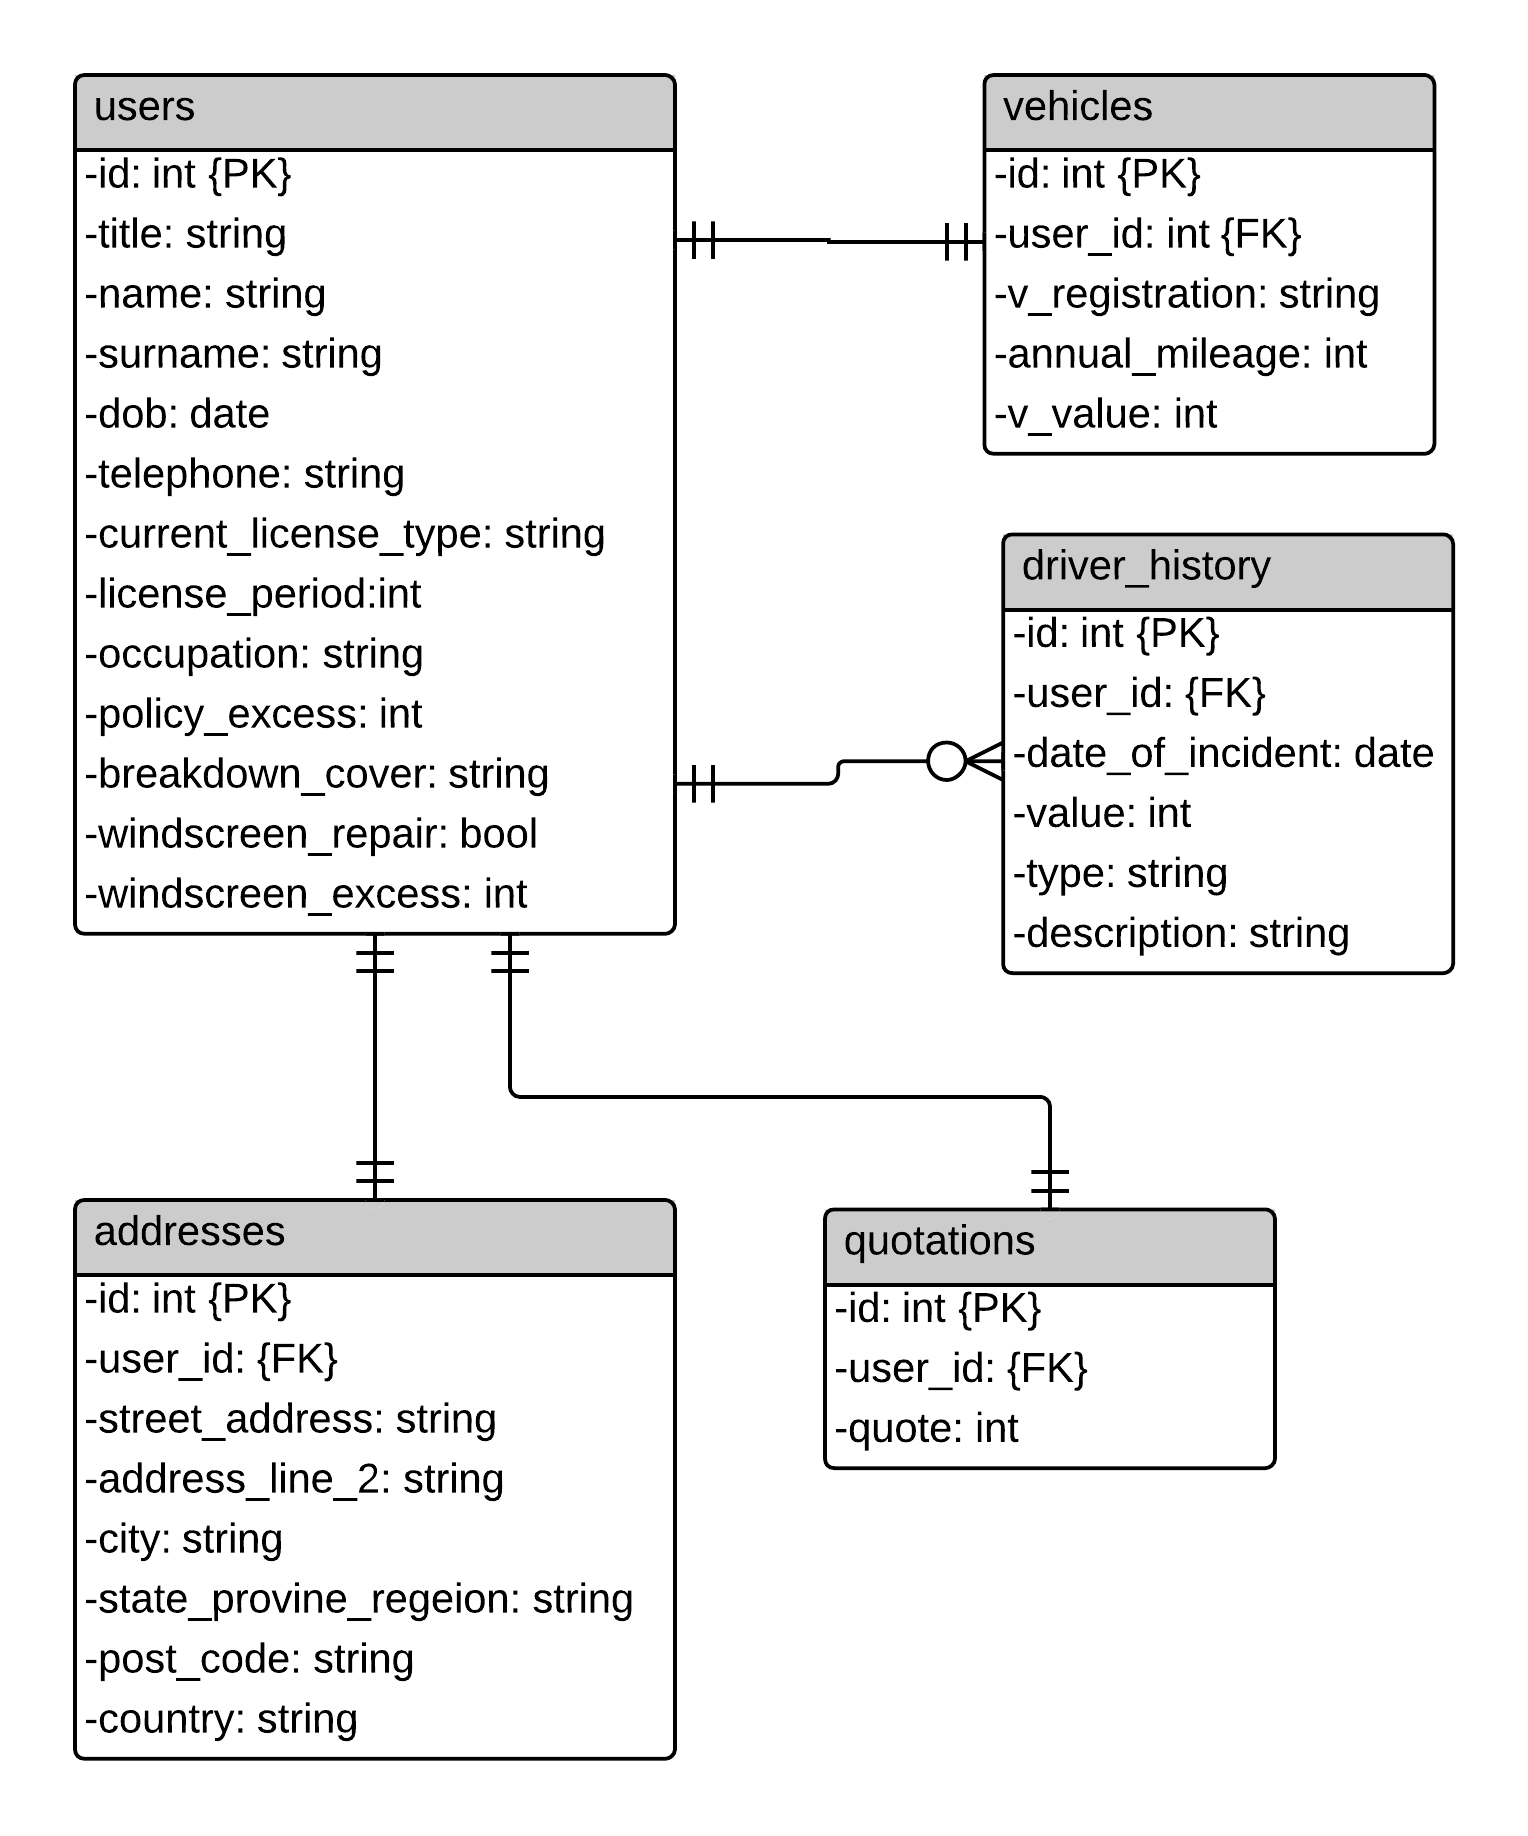
\includegraphics[scale=0.198]{./DatabaseDesign}}
\caption{Database Design}
\label{fig:DatabaseDesign}
\end{figure}

On the figure ~\ref{fig:ClassDesign} there is class diagram of the underwriter application. It is intended to be used as business-to-business application and instead of generating HTML pages interaction is done using data formatted in JSON format and expected to be used by automated clients. As you can see there is nothing under "view" in class diagram since it responds only to data encoded in JSON format (HTML support was left for the debugging purpose to see what is held in the database, but in production mode it would be removed). To create new user broker submits PUT request to the \textit{/users/new.json} address, users controller handles this request and as a response it sends back ID, that was assigned to the newly created user, encoded as JSON. I used ID field in users table as unique reference number for the later quote retrieval. ID field is handled by rails itself and is guaranteed to be unique across all the users so I think it is good way to identify user in the future when the quote needs to be redisplayed. 

\begin{figure}[H]
\centering
\centerline{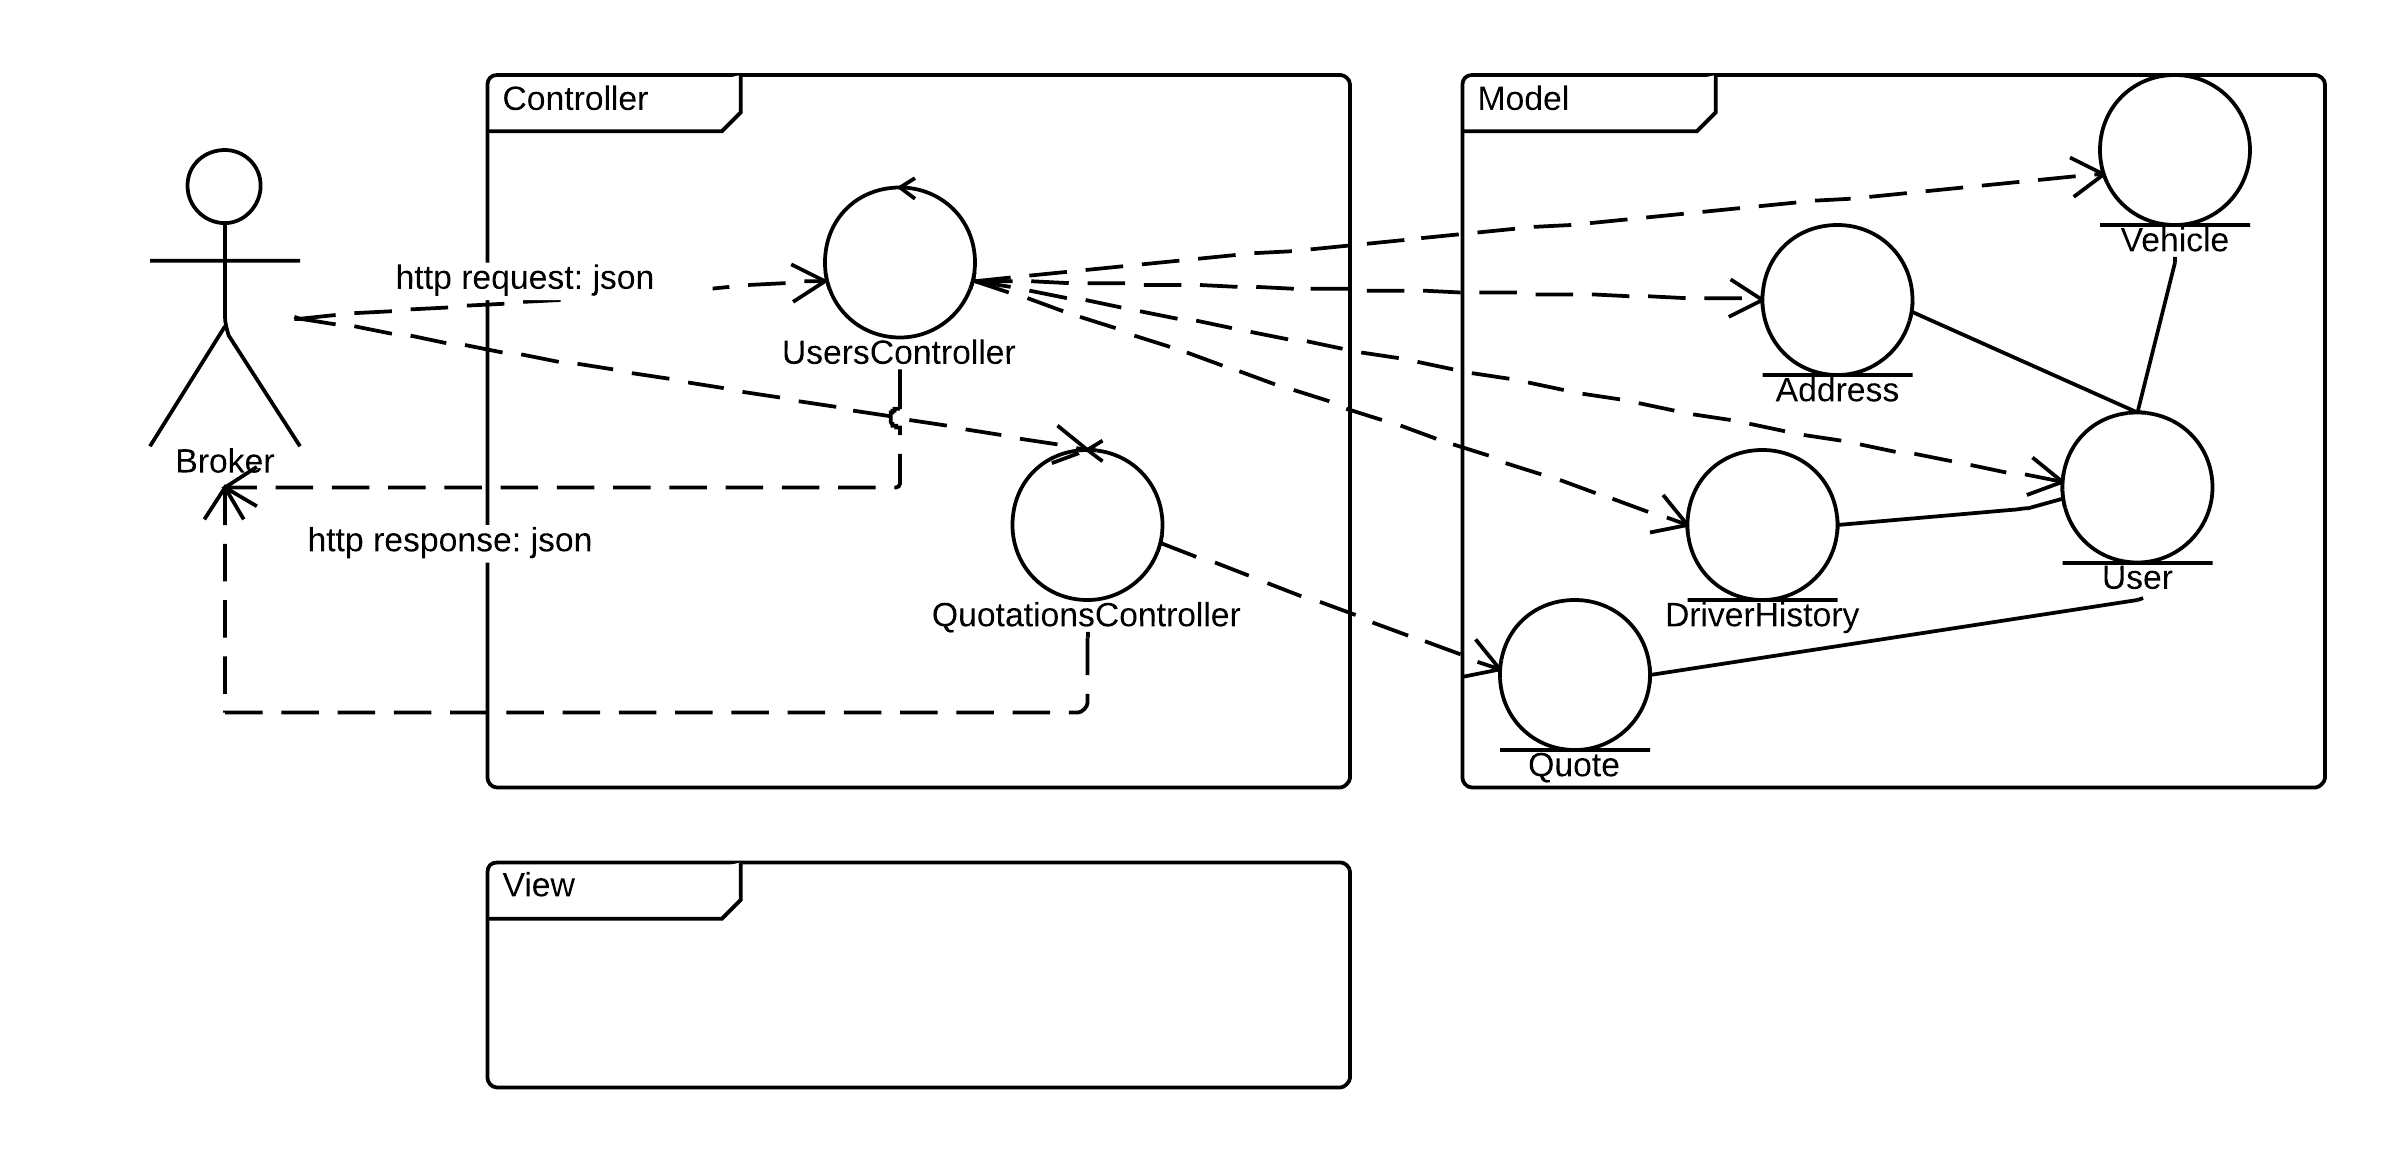
\includegraphics[scale=0.25]{./ClassDesign}}
\caption{Class Diagram}
\label{fig:ClassDesign}
\end{figure}



\section{Architecture of the RESTful broker}
Broker application was written as a web based application with PHP support. It also uses cURL command line tool since it seems to be the only way to send JSON encoded data to the specific URL in the PHP. cURL is produced by the cURL computer software project and allows to transfer data using various protocols \cite{cURL}. My server side scripting experience is limited to the use of SSI in HTML web pages. The fact that PHP is one of the most popular languages used for the server side coding \cite{PHP} seemed to be enough to give it a try. I had no experience in writing PHP code at all so I thought it would be nice to learn it as well. After a few online tutorials I understood basic concepts and started implementing my broker application.

Broker web application provides the ability for the potential customer to request a quote premium from the underwriter application (use case diagram is presented on the figure ~\ref{fig:usecase}). Customer interacts with the broker only via HTTPS and the HTML formatted documents are transmitted to them. On the web page itself customer needs to fill in and submit a form, on the next page user is presented with the amount that it will cost to buy insurance for the car. This quote can be saved for the later retrieval, customer is presented with the unique number which can be used for it. It also provides a web page where unique number can be entered and quote will be redisplayed. Forms used in my web site were generated by the online form generator tool and modified accordingly to suite my needs. PHP is used to get data from the forms and later on in build JSON objects containing customer data. With cURL help broker application then uses standard HTTP methods to communicate with the underwrite application. To get quotation broker preforms PUT request to the \textit{/users/new.json} address and as the response it receives ID number assigned to that user in database. At the next step broker uses received ID to retrieve quotation from the underwriter using GET request and displays it to the user.


\begin{figure}[H]
\centering
\centerline{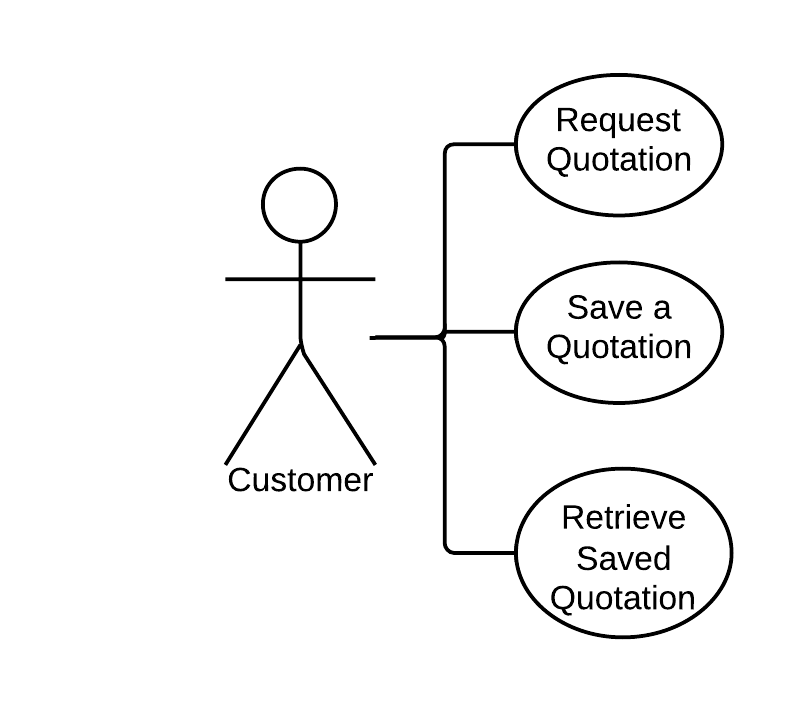
\includegraphics[scale=0.25]{./usecase}}
\caption{Use Case Diagram}
\label{fig:usecase}
\end{figure} 
\section{Test strategy}
Write a section on your test strategy. IMPORTANT: Provide a
screencast of your underwriter application and RESTful broker client
working (some free screen-casting tools can be found online). This
must focus on the broker to underwriter interworking and be no longer
than five minutes long.

\begin{center}
\begin{tabular}{ p{0.2cm} | l | l | l | l | l | l }
   \hline                        
   ID &  Requirement & Description &  Inputs   &  Expected outputs & Pass/Fail & Comments  \\ \hline
   4 & 5 & 6 \\ \hline
   7 & 8 & 9 \\ 
   \hline  
\end{tabular}
\end{center}
\section{Self-evaluation}
Write a self-evaluation section. Say what mark you should be awarded
and why. Say what you found hard or easy, and what was omitted and
why. Provide an analysis of your design and the appropriateness, or
otherwise, of the technologies used.

\bibliographystyle{ieeetr}
\bibliography{bibl}

\end{document}